%% ---- sezione D: setup+risultati ----
\section{Architetture e setup sperimentale}

\paragraph{Benchmark lineari.} La PCA (\S6.1) è addestrata sul solo Training Set standardizzato con $K \in \{3, 10, 20, 100\}$. L'AE lineare (\S6.2) ha un solo layer denso per encoder e decoder, attivazione identità, senza bias né weight decay, ed è ottimizzato sull'MSE con Adam (lr $10^{-3}$, batch 64, fino a 5000 epoche) così da convergere alla PCA.

\paragraph{Autoencoder profondo.} L'AE profondo (\S6.3) adotta un imbuto $65\,703 \to 2048 \to 1024 \to 512 \to K$ con decoder speculare, LeakyReLU ($\alpha = 0.01$) sugli strati nascosti, proiezione latente e layer di uscita lineari. La Tanh in uscita è disattivata perché la sua saturazione agli estremi $\pm 1$ rischia di annullare il gradiente, e il vincolo a $[-1, 1]$ è demandato al clipping finale.

\paragraph{VAE.} Il VAE (\S6.4) condivide l'imbuto, ma il bottleneck si biforca in due teste $\mu$ e $\log \sigma^2$; il codice è campionato con il reparameterization trick ($\mathbf{z} = \mu + \sigma \odot \epsilon$, $\epsilon \sim \mathcal{N}(0, I)$) e in valutazione si pone $\mathbf{z} = \mu$. La loss è $\mathcal{L} = \mathcal{L}_{\text{Recon}} + \beta\,\mathcal{L}_{\text{KL}}$ con $\beta = 1$, poiché entrambi gli addendi sono costruiti da divergenze di Kullback-Leibler e sono dunque grandezze omogenee. Il termine $\mathcal{L}_{\text{Recon}}$ è la divergenza di Jeffreys fra $\mathcal{N}(0, R_{\text{orig}})$ e $\mathcal{N}(0, R_{\text{recon}})$, calcolata nel dominio delle correlazioni dopo la ricomposizione di Cholesky nel grafo differenziabile:
\[
\mathcal{L}_{\text{Recon}} = \tfrac{1}{2}\big[\operatorname{Tr}(R_{\text{recon}}^{-1} R_{\text{orig}}) + \operatorname{Tr}(R_{\text{orig}}^{-1} R_{\text{recon}}) - 2N\big].
\]
Le inverse pesano l'errore in termini relativi su tutto lo spettro, dove l'MSE è cieco agli autovalori più piccoli, e la simmetrizzazione equipara sovrastima e sottostima.

\paragraph{Protocollo e metriche.} Il VAE segue il protocollo della Tabella~6.1 (1000 epoche, batch 64, Adam con lr $10^{-3}$ e weight decay $10^{-5}$, Cosine Annealing, seme 42); l'AE profondo adotta lo stesso schema (tipicamente 1000 epoche, Adam, Cosine Annealing, batch 64; \S6.3). Per entrambi il checkpoint conserva i pesi al minimo assoluto della Validation Loss (\S6.5). Oltre a MSE, MAE e norma di Frobenius, la valutazione impiega cinque metriche topologiche sul Minimum Spanning Tree: edge overlap, indice di Jaccard, scarto della average path length pesata e non pesata, sovrapposizione dei nodi a più alta betweenness.

\section{Risultati: compressione e ricostruzione storica}

\paragraph{Convergenza dei modelli lineari.} In linea con il teorema di Bourlard e Kamp (1988), sul Training Set l'AE lineare converge verso l'MSE della PCA a parità di $K$ (scarto relativo inferiore al 20\%; \S7.1). Sul Test Set i due lineari restano molto vicini, con un vantaggio marginale e sistematico della PCA sulle metriche di errore (\S7.2.1) e valori di fatto sovrapponibili su quelle topologiche (\S7.2.2).

\paragraph{Il vantaggio della non linearità.} L'AE profondo supera nettamente i lineari a ogni $K$, senza segni di overfitting: a $K = 20$ l'MSE di test è $0.72 \times 10^{-4}$ contro $2.73 \times 10^{-4}$ della PCA, con lo stesso ordinamento su MAE e norma di Frobenius (\S7.2.1). Il divario si chiude al crescere di $K$ (Frobenius 20.88 contro 4.22 a $K = 3$, 2.85 contro 2.75 a $K = 100$): è un vantaggio di efficienza rappresentativa, poiché l'AE a $K = 10$ raggiunge la qualità della PCA a $K = 100$ (MAE $0.55 \times 10^{-2}$ per entrambi). La curva dell'AE ha un gomito fra $K = 10$ e $K = 20$ (MSE da $0.84$ a $0.72 \times 10^{-4}$, poi $0.73 \times 10^{-4}$ a $K = 100$), da cui $K = 20$ come compromesso metodologico per il VAE.

\paragraph{Metriche topologiche.} Sull'MST lo stesso ordinamento si ripresenta in forma più netta (\S7.2.2). A $K = 3$ i lineari subiscono un crollo topologico: la PCA conserva il 53.7\% degli archi (Jaccard 37.4\%) contro l'87.7\% (78.5\%) dell'AE; a $K = 100$ i tre modelli deterministici convergono sul 90--91\%, che appare un tetto strutturale. Il VAE a $K = 20$ è intermedio su tutte e cinque le metriche, più vicino all'AE (edge overlap 88.4\% contro 83.0\% della PCA e 91.1\% dell'AE), con la cautela dovuta alle metriche più rumorose (Tabella~\ref{tab:k20}, Figura~\ref{fig:mse_mst}).

\begin{table}[htbp]
\centering\small
\begin{tabular}{lccc}
\toprule
Modello & MSE ($\times 10^{-4}$) & MAE ($\times 10^{-2}$) & Edge overlap MST (\%) \\
\midrule
PCA & 2.73 & 1.18 & 83.0 \\
AE lineare & 3.38 & 1.33 & 83.1 \\
AE profondo & 0.72 & 0.51 & 91.1 \\
VAE & 1.55 & 0.86 & 88.4 \\
\bottomrule
\end{tabular}
\caption{Confronto dei quattro modelli a $K = 20$ sul Test Set (dominio Cholesky): errore di ricostruzione (MSE, MAE) e percentuale di archi dell'MST conservati. I valori sono medie sulle 42 matrici del Test Set, tratti dalle Tabelle 7.1 e 7.2 della tesi.}
\label{tab:k20}
\end{table}

\begin{figure}[htbp]
\centering
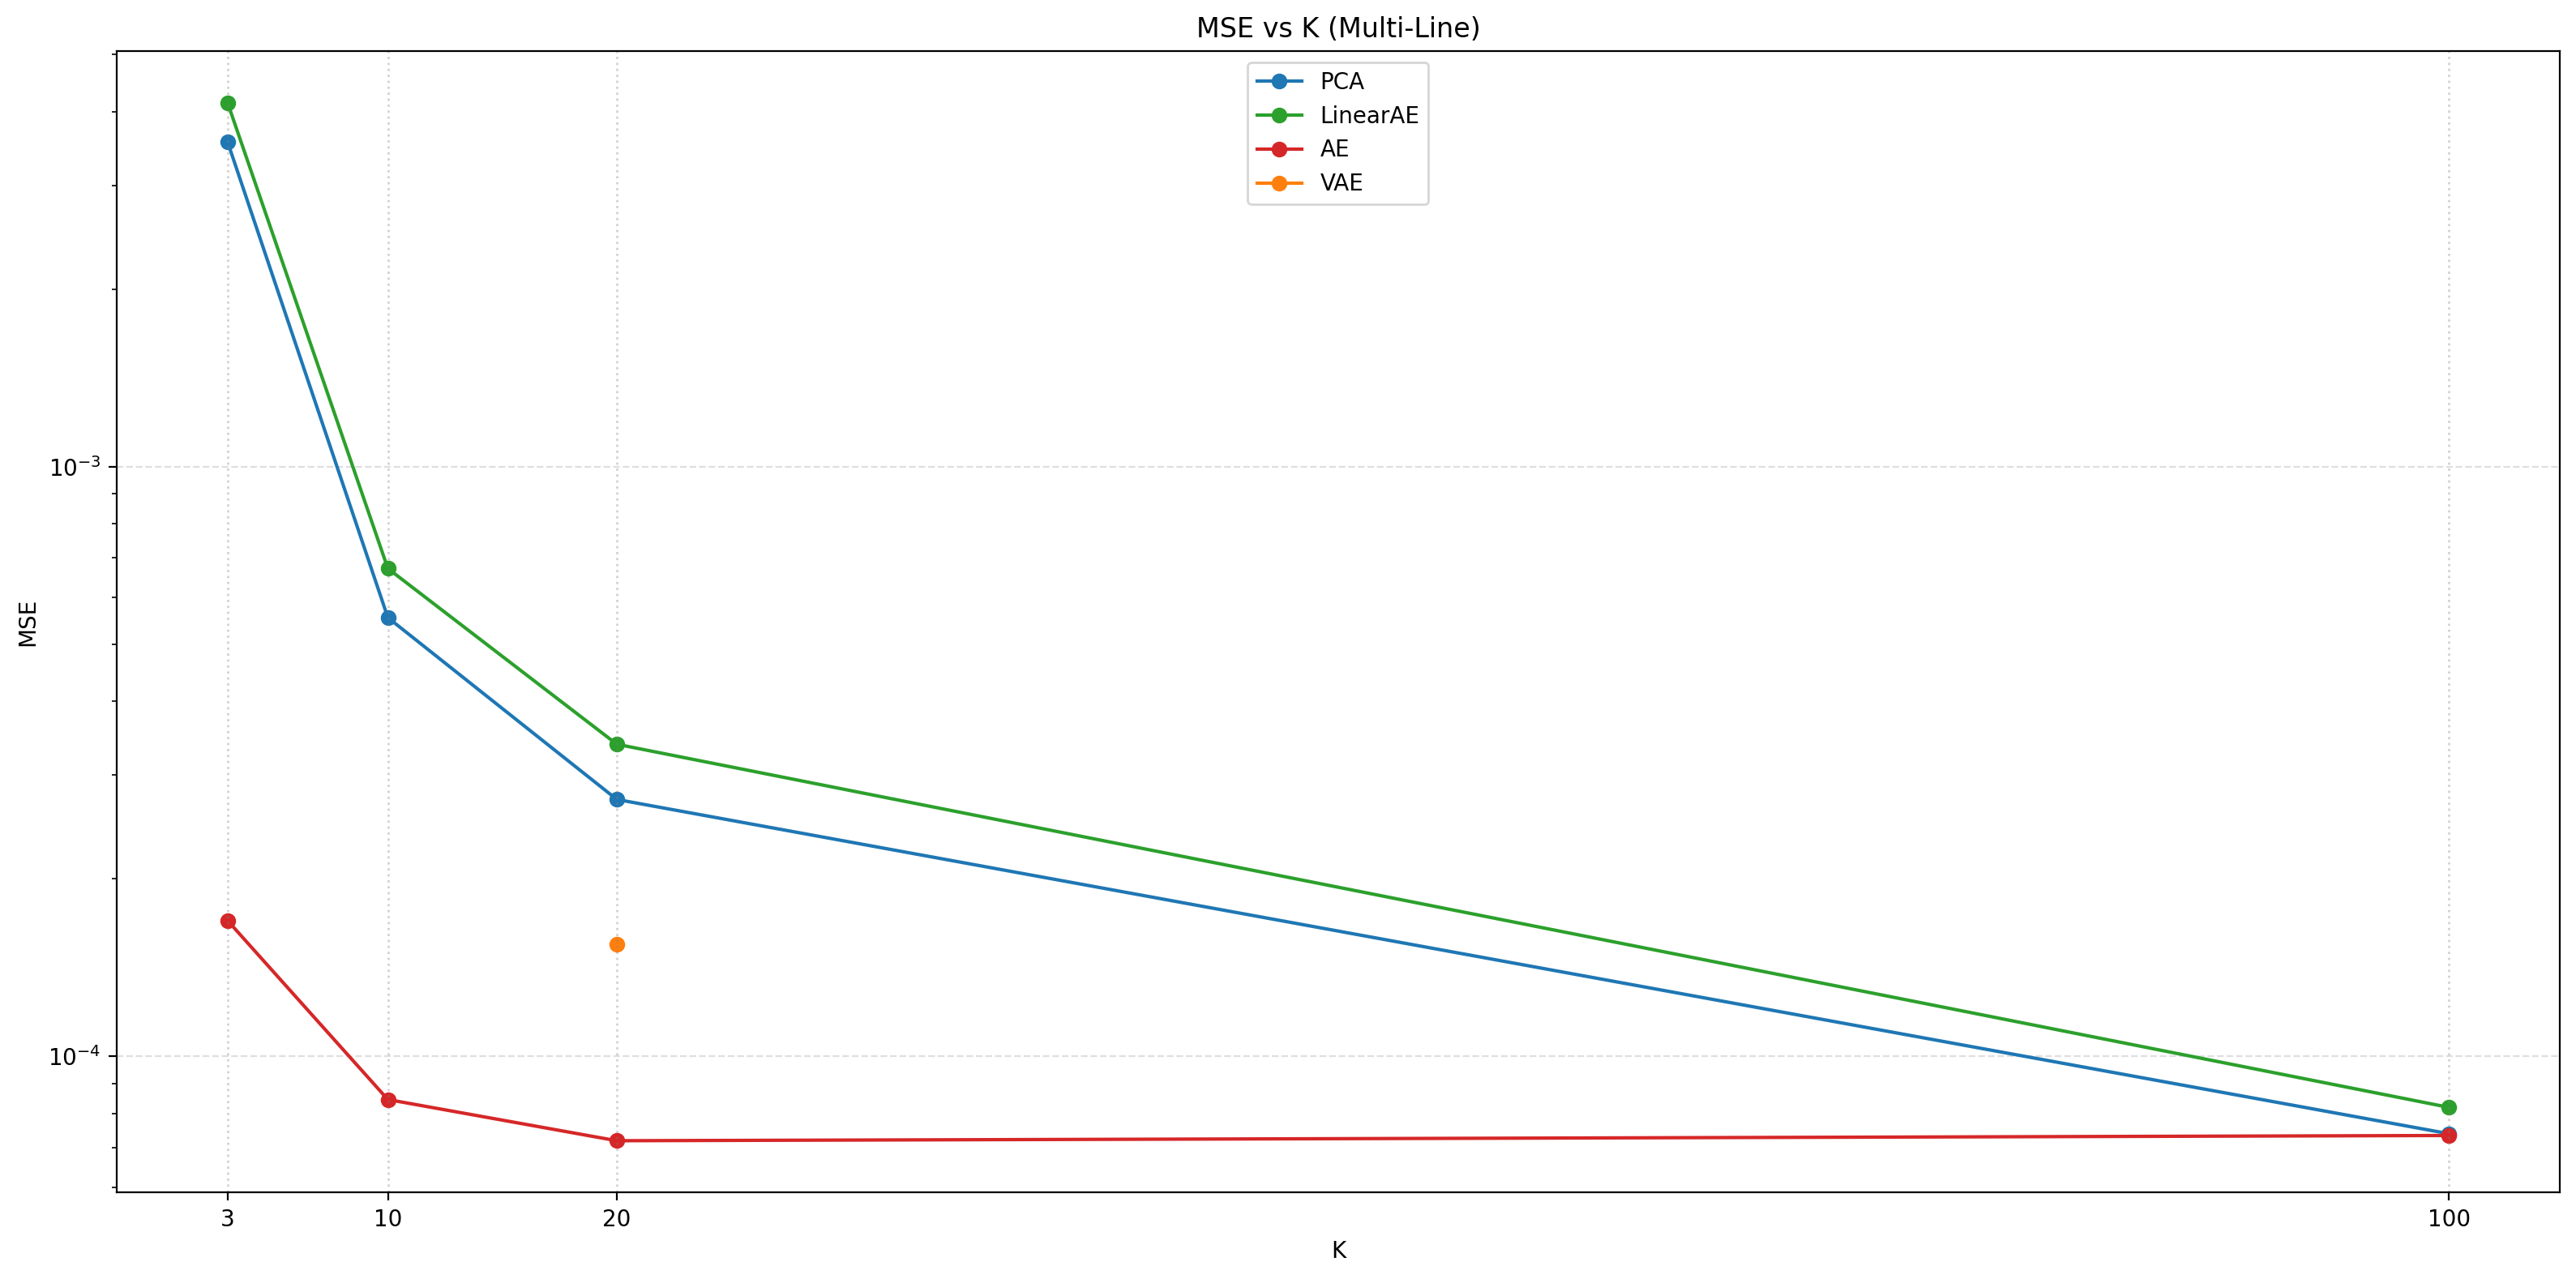
\includegraphics[width=0.84\linewidth]{Pictures/capitolo7/fig_mse_vs_k.png}\par\vspace{5pt}
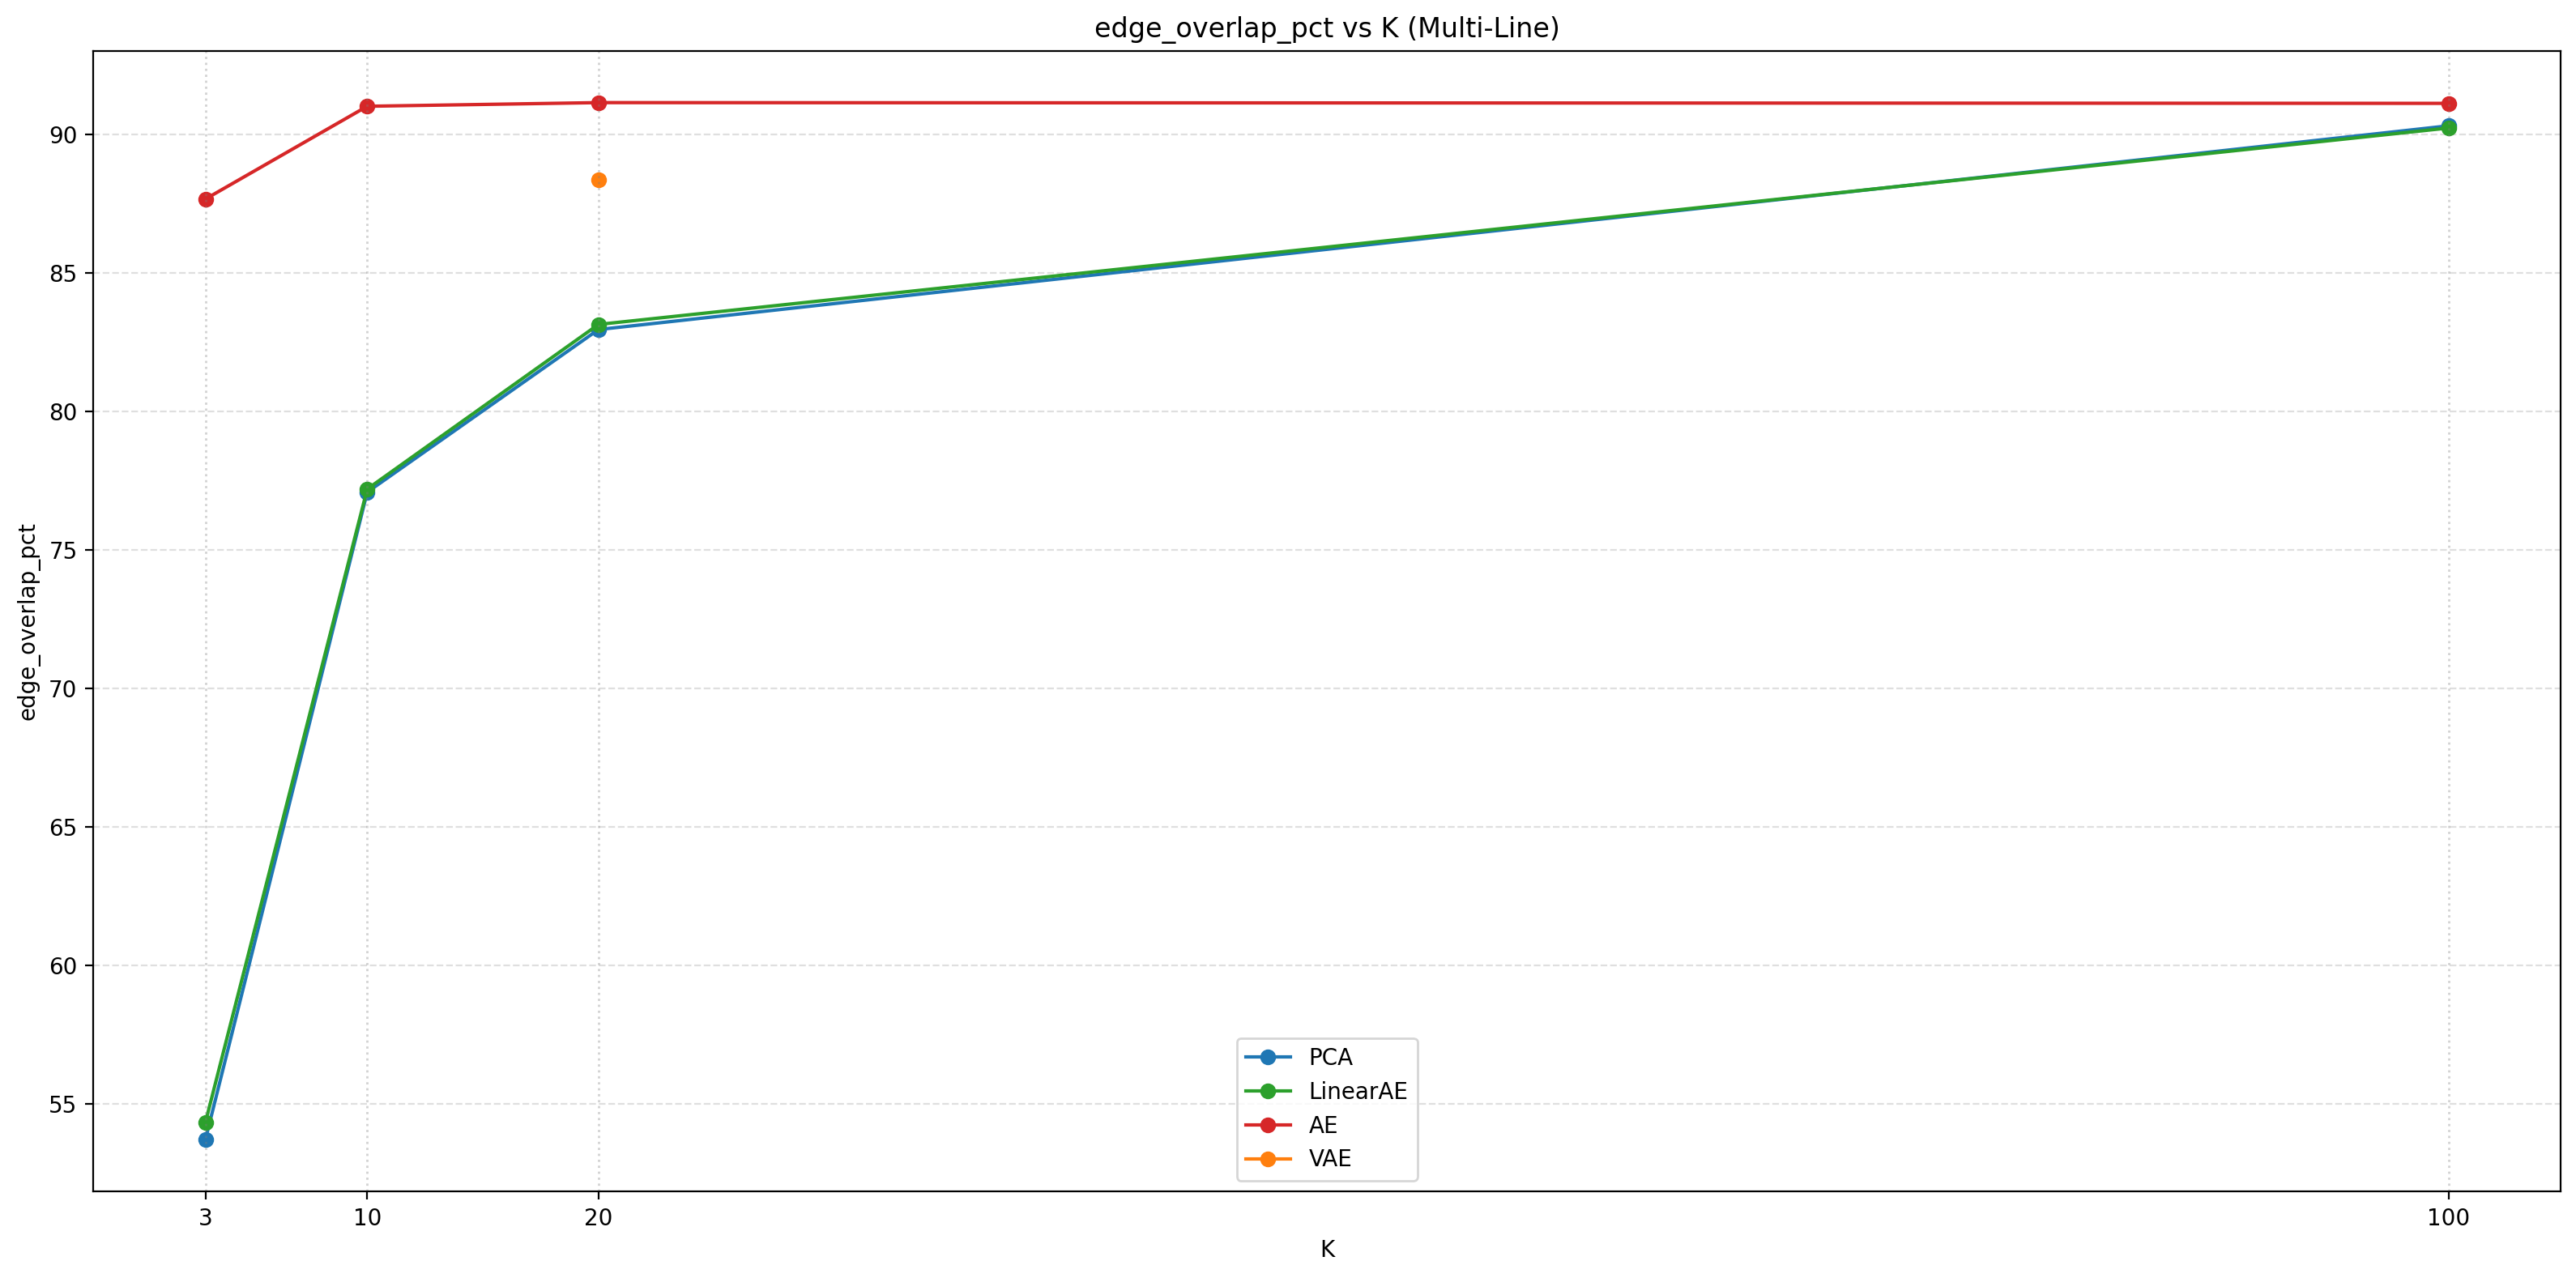
\includegraphics[width=0.84\linewidth]{Pictures/capitolo7/fig_mst_edge_overlap_vs_k.png}
\caption{Errore di ricostruzione MSE (in alto) e percentuale di archi dell'MST conservati (in basso) sul Test Set al variare di $K$ per PCA, AE lineare, AE profondo e VAE (quest'ultimo solo a $K = 20$).}
\label{fig:mse_mst}
\end{figure}

\paragraph{Il VAE al variare di $K$.} Le run a $K = 10$, 20 e 30, identiche salvo $K$ (Tabella~7.3), mostrano un MSE che peggiora con $K$ (da $1.26 \times 10^{-4}$ a $1.88 \times 10^{-4}$), comportamento opposto agli altri modelli, coerente con la competizione fra ricostruzione e termine KL. Le metriche topologiche sono di fatto invarianti (edge overlap 88.6, 88.4 e 88.2\%) e le dimensioni attive con varianza $\geq 0.5$ sono sei in tutte le run: la dimensionalità effettiva appare una proprietà dei dati e la scelta di $K$ poco critica.

\paragraph{Addestramento e spazio latente.} Training e Validation Loss restano allineate fino a circa l'epoca 600. La divergenza di Jeffreys si assesta su un plateau di 7--8 e la KL scende da circa 10 a circa 8, senza divergere né tendere a zero, coerentemente con l'assenza di un collasso globale (\S7.2.4). Lo spettro di varianza dei codici $\mathbf{z} = \mu$ (Figura~\ref{fig:latent}) mostra circa sei dimensioni fortemente attive ($Z_{18}$, $Z_9$, $Z_7$, $Z_1$, $Z_4$, $Z_5$), tre intermedie ($Z_6$, $Z_{10}$, $Z_{12}$) e le restanti in posterior collapse. Le quattro più attive tracciano una manifold continua in cui Training, Validation e Test Set si sovrappongono. Il sottospazio effettivo ha 6--9 dimensioni e quelle in eccesso tendono a collassare, il che offre una chiave di lettura del fatto che l'errore del VAE non decresca con $K$ (\S7.3.1).

\begin{figure}[htbp]
\centering
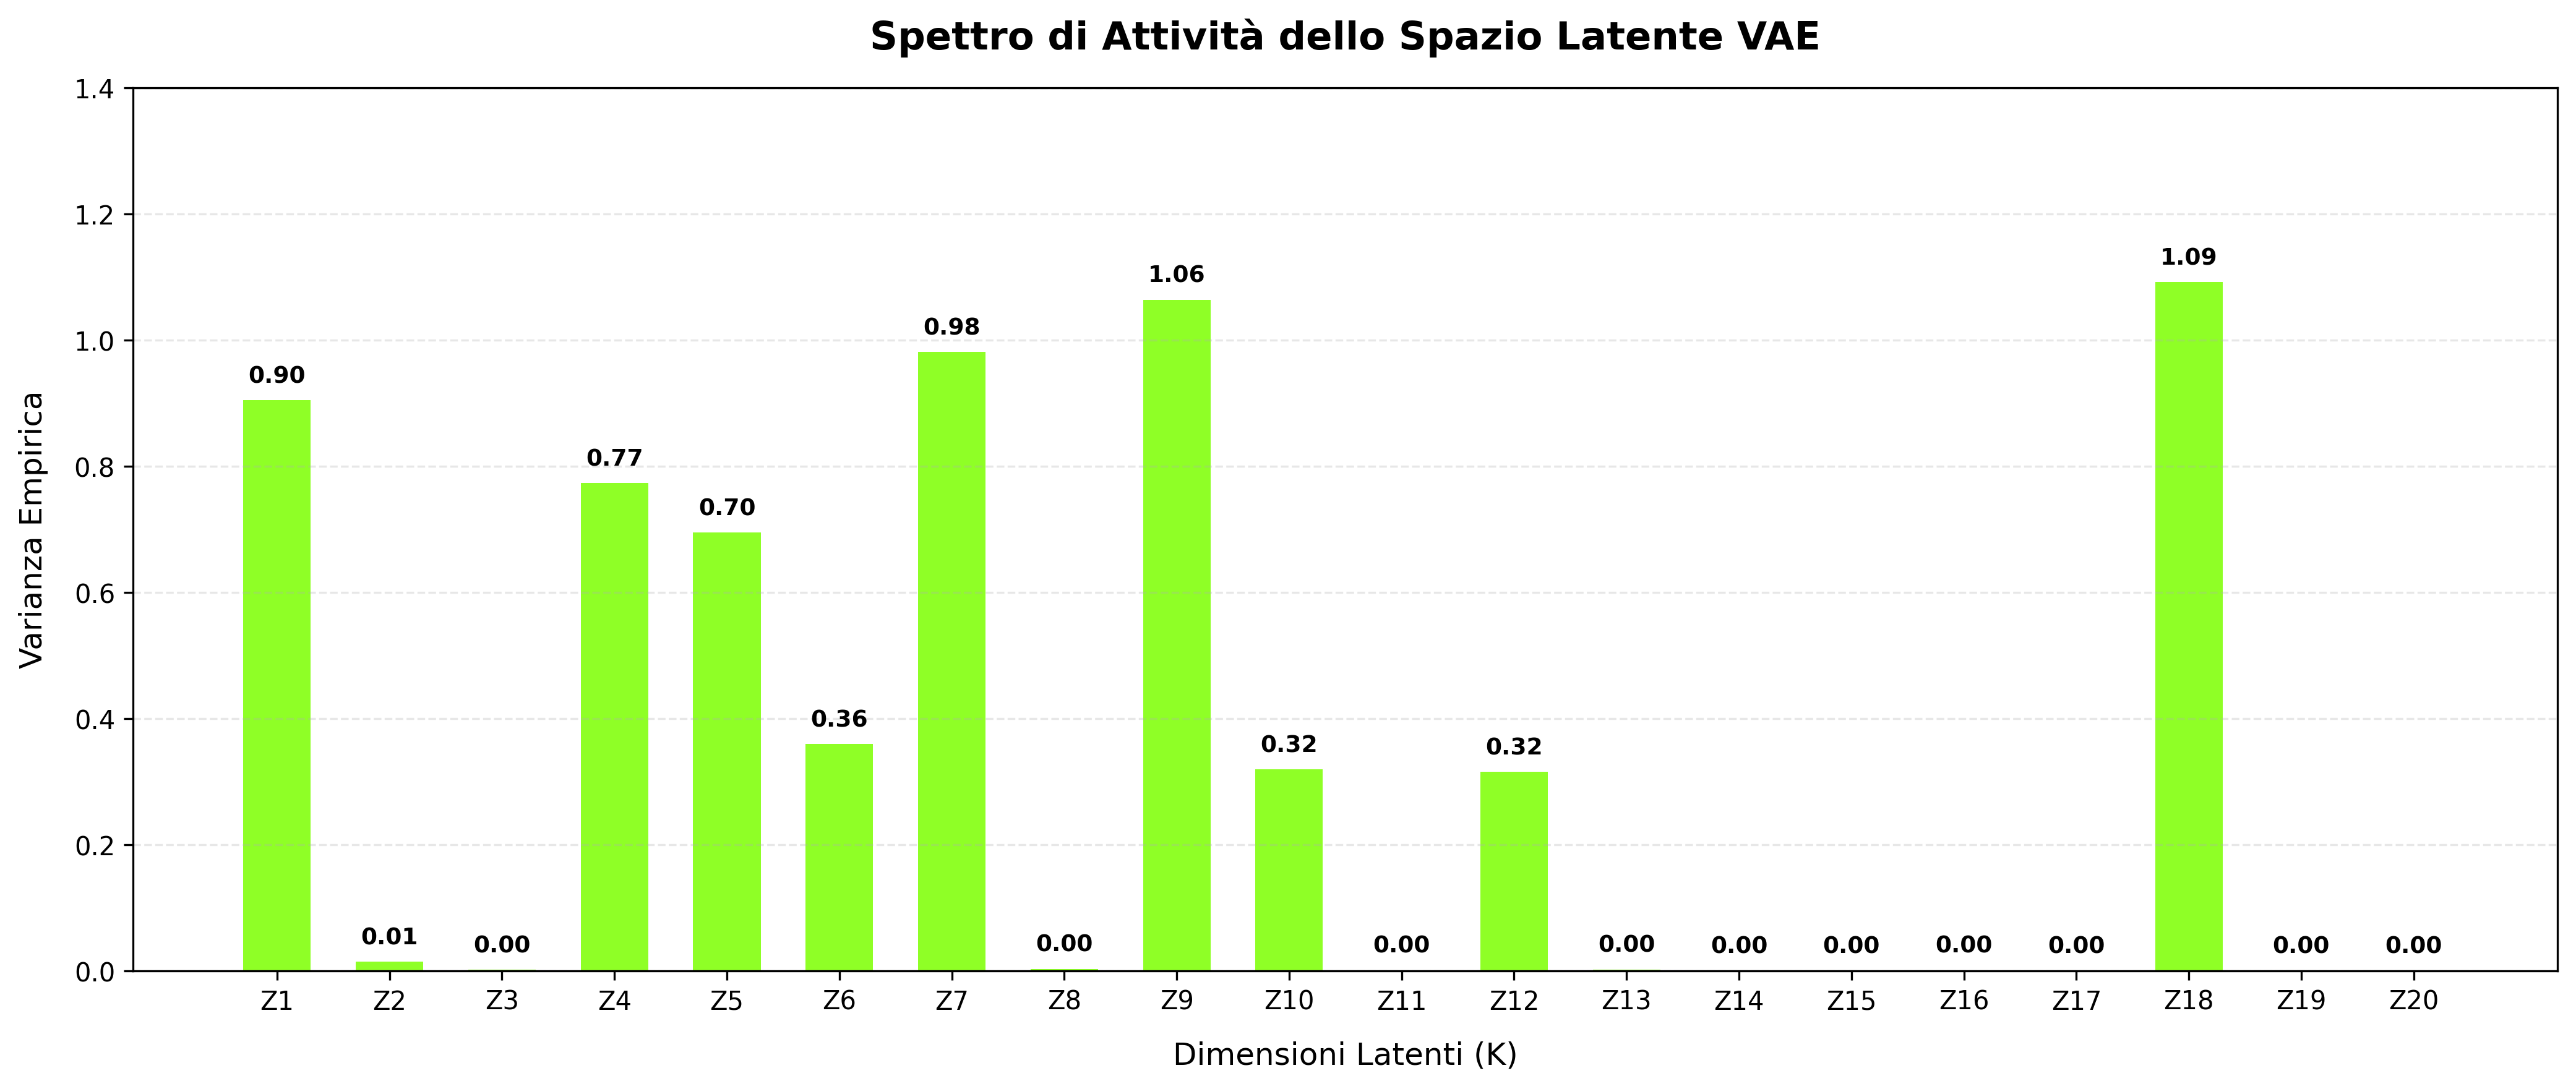
\includegraphics[width=0.9\linewidth]{Pictures/capitolo7/fig_vae_latent_variance_spectrum.png}
\caption{Varianza empirica dei codici latenti $\mathbf{z} = \mu$ delle 288 matrici di training per ciascuna delle 20 dimensioni del VAE definitivo.}
\label{fig:latent}
\end{figure}

\paragraph{Il trade-off.} Il VAE è lievemente meno accurato dell'AE profondo ma superiore ai lineari anche in pura ricostruzione (\S7.3). Il limite dell'AE deterministico, già richiamato, non sta nella qualità della compressione ma in un obiettivo di addestramento che non prevede il campionamento di nuovi punti latenti (premessa metodologica, non esito verificato sperimentalmente). In cambio di uno scarto contenuto, la regolarizzazione variazionale del VAE modella uno spazio latente continuo e denso in cui campionare: per questo è il modello scelto per generare gli scenari.
